\section{Geometry}
\label{sec:background}


\begin{figure}[ht]
\centering
\begin{minipage}{.5\textwidth}
  \centering
  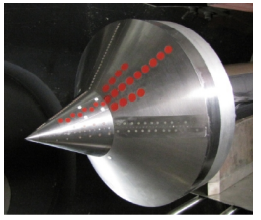
\includegraphics[width=0.9\linewidth]{images/doublecone.png}
  \caption{ Double cone geometric dimensions in mm [3].}
  \label{fig:ExperimentCone}
\end{minipage}%
\begin{minipage}{.5\textwidth}
  \centering
 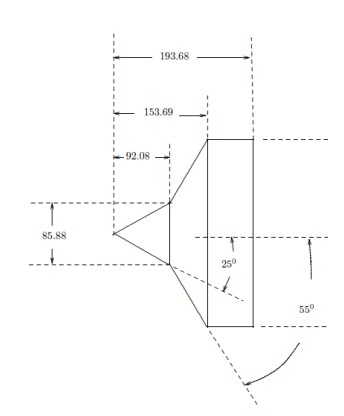
\includegraphics[width =0.9\linewidth]{images/model_dimensions.jpg}
  \caption{ Double cone configuration C [4].}
  \label{fig:ModelDimensions}
\end{minipage}
\end{figure}

\begin{figure}[ht]
\centering
  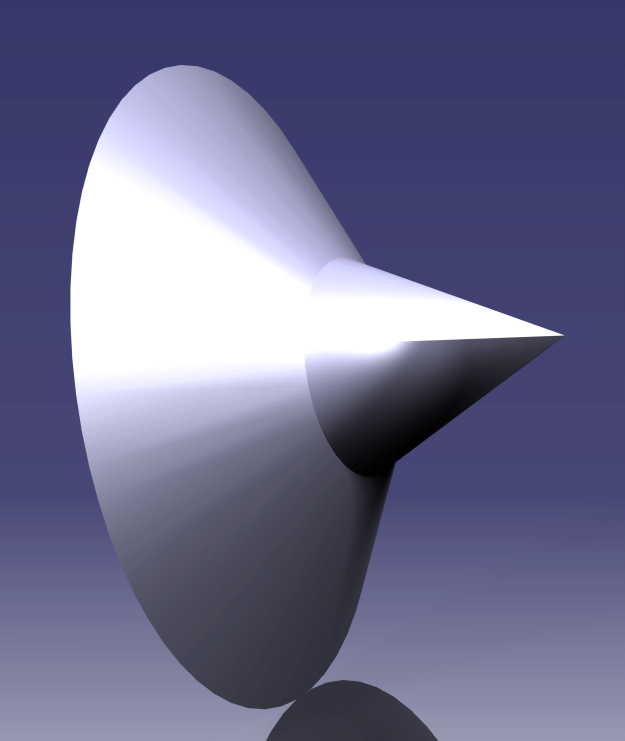
\includegraphics[width=0.4\linewidth]{images/CONE.jpg}
  \caption{ Double Cone model designed using CATIA V5.}
  \label{fig:CATIA_CONE}
\end{figure}

The Double cone configuration was designed from [3] and depicted in Figure \ref{fig:ModelDimensions} with forward and aft angles of $25^\circ$ and $55^\circ$
respectively, The heat transfer and pressure sensor location are placed in the front nose or the forward cone which is depicted in Figure \ref{fig:ExperimentCone}, The overall length of the cone is 193.68 mm with overall height of 126.164 mm.